 \documentclass{article}
\usepackage[utf8]{inputenc}
\usepackage[a4paper, total={7in, 10in}]{geometry}
\usepackage{braket}
\usepackage{xcolor}
\usepackage{amsmath}
\usepackage{amssymb}
\usepackage{amsfonts}
\usepackage{graphicx}
\usepackage{svg}
\usepackage{float}
\usepackage{tikz}
\usepackage[ruled,vlined]{algorithm2e}
\usepackage{multicol}
\usepackage[backend=biber,style=alphabetic,sorting=ynt]{biblatex}
\usepackage{xcolor}
%\addbibresource{sample.bib} %Import the bibliography file

\newcommand{\commentt}[1]{\textcolor{blue}{ \textbf{[COMMENT]} #1}}
\newcommand{\ctt}[1]{\commentt{#1}}
\newcommand{\prb}[1]{ \mathbf{Pr} \left[ {#1} \right]}
\newcommand{\onotation}[1]{\(\mathcal{O} \left( {#1}  \right) \)}
\newcommand{\ona}[1]{\onotation{#1}}
\newcommand{\PSI}{{\ket{\psi}}}
\newcommand{\LESn}{\ket{\psi_n}}
\newcommand{\LESa}{\ket{\phi_n}}
\newcommand{\LESs}{\frac{1}{\sqrt{n}}\sum_{i}{\ket{\left(0^{i}10^{n-i}\right)^{n}}}}
\newcommand{\Hn}{\mathcal{H}_{n}}
\newcommand{\Ep}{\frac{1}{\sqrt{2^n}}\sum^{2^n}_{x}{ \ket{xx}}}
\newcommand{\HON}{\ket{\psi_{\text{honest}}}}
\newcommand{\Lemma}{\paragraph{Lemma.}}


\setlength{\columnsep}{0.6cm}

\newcommand{\Gz}{ G_{z}^{\delta} } 

\begin{document}

\title{Quantum LTC With Positive Rate}
\author{David Ponarovsky}
\maketitle
\begin{multicols*}{2}
\newcommand{ \Hw }{ \delta\Delta -\Delta^{\frac{1}{2}-\varepsilon}/\delta  }
	\newcommand{ \Nw }{ \Delta^{\frac{3}{2}-\varepsilon}} 
	  \newcommand{ \Gu } { \Gamma^{\cup} }
	  \newcommand{ \Guq } { \Gamma^{\cup, \square} }

    	\newcommand{ \Gsa } {\Gamma_{\square_{1}} }
	\newcommand{ \Gsb } {\Gamma_{\square_{2}} }
        \newcommand{ \Aa } { C_{A_{1}}}  
	\newcommand{ \Ab } { C_{A_{2}}}
	\newcommand{ \Ac } { C_{A_{3}}}
	\newcommand{ \Aab } { \Aa \otimes \Ab } 
	\newcommand{ \Aac } { \Aa \otimes \Ac }
	\newcommand{ \Aabc } { \Aa \otimes \Ab \otimes \Ac }
	\newcommand{ \Aabp } { \Aa^{\perp} \otimes \Ab^{\perp} } 
	\newcommand{ \Aacp } { \Aa^{\perp} \otimes \Ac^{\perp} }
	\newcommand{ \Aabcp } { \Aa^{\perp} \otimes \Ab^{\perp} \otimes \Ac^{\perp} }
	\newcommand{ \Aabpp } { \left( \Aabp \right)^\perp } 
	\newcommand{ \Aacpp } { \left( \Aacp \right)^\perp }
	\newcommand{ \Aabcpp } { \left( \Aabcp \right)^\perp }
	\newcommand{ \YY } {  y_{1}y_{2}^{\top} }
	\newcommand{ \ZZ } {  z_{1}z_{2}^{\top} } 
	\newcommand{ \TT } { \tilde{\tau} } 


  \paragraph{preamble.} preamble.  
  \begin{figure}[H]
            %\label{fig:square}
            \begin{center}
            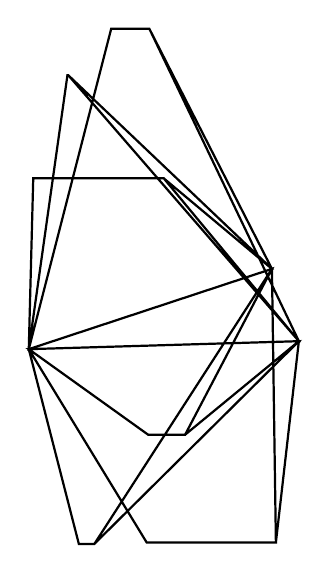
\begin{tikzpicture}
            \draw[thick](0,0)(0,0)  -- (0.4908246384464048, 3.4778770865824327) -- (0.5026434015958758, 3.4778770865824327) -- (3.43000913992395,0.10127194810436166) -- (0,0) -- (0,0)  -- (1.5166070901634243, -1.0868798383210798) -- (1.9849570127830862, -1.0868798383210798) -- (3.43000913992395,0.10127194810436166) -- (0,0) -- 
(0,0)  -- (0.4908246384464048, 3.4778770865824327) -- (0.5026434015958758, 3.4778770865824327) -- (3.43000913992395,0.10127194810436166) -- (0,0) -- (0,0)  -- (0.6361986155480959, -2.47477097489175) -- (0.8320020754304234, -2.47477097489175) -- (3.43000913992395,0.10127194810436166) -- (0,0) -- 
(0,0)  -- (0.4908246384464048, 3.4778770865824327) -- (0.5026434015958758, 3.4778770865824327) -- (3.43000913992395,0.10127194810436166) -- (0,0) -- (0,0)  -- (1.4969928612496044, -2.4545457009443923) -- (3.138343491448329, -2.4545457009443923) -- (3.43000913992395,0.10127194810436166) -- (0,0) -- 
(0,0)  -- (0.05663882096812456, 2.1694579437706794) -- (1.714304980551444, 2.1694579437706794) -- (3.43000913992395,0.10127194810436166) -- (0,0) -- (0,0)  -- (1.5166070901634243, -1.0868798383210798) -- (1.9849570127830862, -1.0868798383210798) -- (3.43000913992395,0.10127194810436166) -- (0,0) -- 
(0,0)  -- (0.05663882096812456, 2.1694579437706794) -- (1.714304980551444, 2.1694579437706794) -- (3.43000913992395,0.10127194810436166) -- (0,0) -- (0,0)  -- (0.6361986155480959, -2.47477097489175) -- (0.8320020754304234, -2.47477097489175) -- (3.43000913992395,0.10127194810436166) -- (0,0) -- 
(0,0)  -- (0.05663882096812456, 2.1694579437706794) -- (1.714304980551444, 2.1694579437706794) -- (3.43000913992395,0.10127194810436166) -- (0,0) -- (0,0)  -- (1.4969928612496044, -2.4545457009443923) -- (3.138343491448329, -2.4545457009443923) -- (3.43000913992395,0.10127194810436166) -- (0,0) -- 
(0,0)  -- (1.0466060143809082, 4.068804076537469) -- (1.5312977450946816, 4.068804076537469) -- (3.43000913992395,0.10127194810436166) -- (0,0) -- (0,0)  -- (1.5166070901634243, -1.0868798383210798) -- (1.9849570127830862, -1.0868798383210798) -- (3.43000913992395,0.10127194810436166) -- (0,0) -- 
(0,0)  -- (1.0466060143809082, 4.068804076537469) -- (1.5312977450946816, 4.068804076537469) -- (3.43000913992395,0.10127194810436166) -- (0,0) -- (0,0)  -- (0.6361986155480959, -2.47477097489175) -- (0.8320020754304234, -2.47477097489175) -- (3.43000913992395,0.10127194810436166) -- (0,0) -- 
(0,0)  -- (1.0466060143809082, 4.068804076537469) -- (1.5312977450946816, 4.068804076537469) -- (3.43000913992395,0.10127194810436166) -- (0,0) -- (0,0)  -- (1.4969928612496044, -2.4545457009443923) -- (3.138343491448329, -2.4545457009443923) -- (3.43000913992395,0.10127194810436166) -- (0,0) -- 
(0,0)  -- (0.4908246384464048, 3.4778770865824327) -- (0.5026434015958758, 3.4778770865824327) -- (3.0881388886989134,1.019392848987625) -- (0,0) -- (0,0)  -- (1.5166070901634243, -1.0868798383210798) -- (1.9849570127830862, -1.0868798383210798) -- (3.0881388886989134,1.019392848987625) -- (0,0) -- 
(0,0)  -- (0.4908246384464048, 3.4778770865824327) -- (0.5026434015958758, 3.4778770865824327) -- (3.0881388886989134,1.019392848987625) -- (0,0) -- (0,0)  -- (0.6361986155480959, -2.47477097489175) -- (0.8320020754304234, -2.47477097489175) -- (3.0881388886989134,1.019392848987625) -- (0,0) -- 
(0,0)  -- (0.4908246384464048, 3.4778770865824327) -- (0.5026434015958758, 3.4778770865824327) -- (3.0881388886989134,1.019392848987625) -- (0,0) -- (0,0)  -- (1.4969928612496044, -2.4545457009443923) -- (3.138343491448329, -2.4545457009443923) -- (3.0881388886989134,1.019392848987625) -- (0,0) -- 
(0,0)  -- (0.05663882096812456, 2.1694579437706794) -- (1.714304980551444, 2.1694579437706794) -- (3.0881388886989134,1.019392848987625) -- (0,0) -- (0,0)  -- (1.5166070901634243, -1.0868798383210798) -- (1.9849570127830862, -1.0868798383210798) -- (3.0881388886989134,1.019392848987625) -- (0,0) -- 
(0,0)  -- (0.05663882096812456, 2.1694579437706794) -- (1.714304980551444, 2.1694579437706794) -- (3.0881388886989134,1.019392848987625) -- (0,0) -- (0,0)  -- (0.6361986155480959, -2.47477097489175) -- (0.8320020754304234, -2.47477097489175) -- (3.0881388886989134,1.019392848987625) -- (0,0) -- 
(0,0)  -- (0.05663882096812456, 2.1694579437706794) -- (1.714304980551444, 2.1694579437706794) -- (3.0881388886989134,1.019392848987625) -- (0,0) -- (0,0)  -- (1.4969928612496044, -2.4545457009443923) -- (3.138343491448329, -2.4545457009443923) -- (3.0881388886989134,1.019392848987625) -- (0,0) -- 
(0,0)  -- (1.0466060143809082, 4.068804076537469) -- (1.5312977450946816, 4.068804076537469) -- (3.0881388886989134,1.019392848987625) -- (0,0) -- (0,0)  -- (1.5166070901634243, -1.0868798383210798) -- (1.9849570127830862, -1.0868798383210798) -- (3.0881388886989134,1.019392848987625) -- (0,0) -- 
(0,0)  -- (1.0466060143809082, 4.068804076537469) -- (1.5312977450946816, 4.068804076537469) -- (3.0881388886989134,1.019392848987625) -- (0,0) -- (0,0)  -- (0.6361986155480959, -2.47477097489175) -- (0.8320020754304234, -2.47477097489175) -- (3.0881388886989134,1.019392848987625) -- (0,0) -- 
(0,0)  -- (1.0466060143809082, 4.068804076537469) -- (1.5312977450946816, 4.068804076537469) -- (3.0881388886989134,1.019392848987625) -- (0,0) -- (0,0)  -- (1.4969928612496044, -2.4545457009443923) -- (3.138343491448329, -2.4545457009443923) -- (3.0881388886989134,1.019392848987625) -- (0,0) -- 
(0,0);
            \end{tikzpicture}
            \end{center}
            \caption{Square of the complex, with edges $(g,ag), (agb, gb) \in E_A,
            (g,gb), (agb, ag) \in E_B.$ \label{fig:square}
            }
            \end{figure}
 \begin{figure}[H]
            %\label{fig:square}
            \begin{center}
            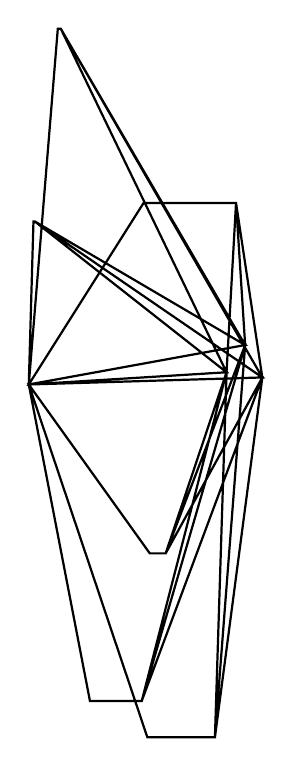
\begin{tikzpicture}
            \draw[thick](0,0)(0,0)  -- (0.36851045735554266, 4.517345380239817) -- (0.40685693643424514, 4.517345380239817) -- (2.9658483129271467,0.08929309063120545) -- (0,0) -- (0,0)  -- (0.7767037334385709, -4.018614714218383) -- (1.4348345974928318, -4.018614714218383) -- (2.9658483129271467,0.08929309063120545) -- (0,0) -- 
(0,0)  -- (0.36851045735554266, 4.517345380239817) -- (0.40685693643424514, 4.517345380239817) -- (2.9658483129271467,0.08929309063120545) -- (0,0) -- (0,0)  -- (1.5368435165972947, -2.1447871397444866) -- (1.7386276054999228, -2.1447871397444866) -- (2.9658483129271467,0.08929309063120545) -- (0,0) -- 
(0,0)  -- (0.36851045735554266, 4.517345380239817) -- (0.40685693643424514, 4.517345380239817) -- (2.9658483129271467,0.08929309063120545) -- (0,0) -- (0,0)  -- (1.5059714394858557, -4.480977099238024) -- (2.3640899012852326, -4.480977099238024) -- (2.9658483129271467,0.08929309063120545) -- (0,0) -- 
(0,0)  -- (0.05945510209784022, 2.070692820415272) -- (0.07609805008402426, 2.070692820415272) -- (2.9658483129271467,0.08929309063120545) -- (0,0) -- (0,0)  -- (0.7767037334385709, -4.018614714218383) -- (1.4348345974928318, -4.018614714218383) -- (2.9658483129271467,0.08929309063120545) -- (0,0) -- 
(0,0)  -- (0.05945510209784022, 2.070692820415272) -- (0.07609805008402426, 2.070692820415272) -- (2.9658483129271467,0.08929309063120545) -- (0,0) -- (0,0)  -- (1.5368435165972947, -2.1447871397444866) -- (1.7386276054999228, -2.1447871397444866) -- (2.9658483129271467,0.08929309063120545) -- (0,0) -- 
(0,0)  -- (0.05945510209784022, 2.070692820415272) -- (0.07609805008402426, 2.070692820415272) -- (2.9658483129271467,0.08929309063120545) -- (0,0) -- (0,0)  -- (1.5059714394858557, -4.480977099238024) -- (2.3640899012852326, -4.480977099238024) -- (2.9658483129271467,0.08929309063120545) -- (0,0) -- 
(0,0)  -- (1.458460903645077, 2.3059745693316835) -- (2.6321265082725125, 2.3059745693316835) -- (2.9658483129271467,0.08929309063120545) -- (0,0) -- (0,0)  -- (0.7767037334385709, -4.018614714218383) -- (1.4348345974928318, -4.018614714218383) -- (2.9658483129271467,0.08929309063120545) -- (0,0) -- 
(0,0)  -- (1.458460903645077, 2.3059745693316835) -- (2.6321265082725125, 2.3059745693316835) -- (2.9658483129271467,0.08929309063120545) -- (0,0) -- (0,0)  -- (1.5368435165972947, -2.1447871397444866) -- (1.7386276054999228, -2.1447871397444866) -- (2.9658483129271467,0.08929309063120545) -- (0,0) -- 
(0,0)  -- (1.458460903645077, 2.3059745693316835) -- (2.6321265082725125, 2.3059745693316835) -- (2.9658483129271467,0.08929309063120545) -- (0,0) -- (0,0)  -- (1.5059714394858557, -4.480977099238024) -- (2.3640899012852326, -4.480977099238024) -- (2.9658483129271467,0.08929309063120545) -- (0,0) -- 
(0,0)  -- (0.36851045735554266, 4.517345380239817) -- (0.40685693643424514, 4.517345380239817) -- (2.748002502447032,0.5008646210616042) -- (0,0) -- (0,0)  -- (0.7767037334385709, -4.018614714218383) -- (1.4348345974928318, -4.018614714218383) -- (2.748002502447032,0.5008646210616042) -- (0,0) -- 
(0,0)  -- (0.36851045735554266, 4.517345380239817) -- (0.40685693643424514, 4.517345380239817) -- (2.748002502447032,0.5008646210616042) -- (0,0) -- (0,0)  -- (1.5368435165972947, -2.1447871397444866) -- (1.7386276054999228, -2.1447871397444866) -- (2.748002502447032,0.5008646210616042) -- (0,0) -- 
(0,0)  -- (0.36851045735554266, 4.517345380239817) -- (0.40685693643424514, 4.517345380239817) -- (2.748002502447032,0.5008646210616042) -- (0,0) -- (0,0)  -- (1.5059714394858557, -4.480977099238024) -- (2.3640899012852326, -4.480977099238024) -- (2.748002502447032,0.5008646210616042) -- (0,0) -- 
(0,0)  -- (0.05945510209784022, 2.070692820415272) -- (0.07609805008402426, 2.070692820415272) -- (2.748002502447032,0.5008646210616042) -- (0,0) -- (0,0)  -- (0.7767037334385709, -4.018614714218383) -- (1.4348345974928318, -4.018614714218383) -- (2.748002502447032,0.5008646210616042) -- (0,0) -- 
(0,0)  -- (0.05945510209784022, 2.070692820415272) -- (0.07609805008402426, 2.070692820415272) -- (2.748002502447032,0.5008646210616042) -- (0,0) -- (0,0)  -- (1.5368435165972947, -2.1447871397444866) -- (1.7386276054999228, -2.1447871397444866) -- (2.748002502447032,0.5008646210616042) -- (0,0) -- 
(0,0)  -- (0.05945510209784022, 2.070692820415272) -- (0.07609805008402426, 2.070692820415272) -- (2.748002502447032,0.5008646210616042) -- (0,0) -- (0,0)  -- (1.5059714394858557, -4.480977099238024) -- (2.3640899012852326, -4.480977099238024) -- (2.748002502447032,0.5008646210616042) -- (0,0) -- 
(0,0)  -- (1.458460903645077, 2.3059745693316835) -- (2.6321265082725125, 2.3059745693316835) -- (2.748002502447032,0.5008646210616042) -- (0,0) -- (0,0)  -- (0.7767037334385709, -4.018614714218383) -- (1.4348345974928318, -4.018614714218383) -- (2.748002502447032,0.5008646210616042) -- (0,0) -- 
(0,0)  -- (1.458460903645077, 2.3059745693316835) -- (2.6321265082725125, 2.3059745693316835) -- (2.748002502447032,0.5008646210616042) -- (0,0) -- (0,0)  -- (1.5368435165972947, -2.1447871397444866) -- (1.7386276054999228, -2.1447871397444866) -- (2.748002502447032,0.5008646210616042) -- (0,0) -- 
(0,0)  -- (1.458460903645077, 2.3059745693316835) -- (2.6321265082725125, 2.3059745693316835) -- (2.748002502447032,0.5008646210616042) -- (0,0) -- (0,0)  -- (1.5059714394858557, -4.480977099238024) -- (2.3640899012852326, -4.480977099238024) -- (2.748002502447032,0.5008646210616042) -- (0,0) -- 
(0,0)  -- (0.36851045735554266, 4.517345380239817) -- (0.40685693643424514, 4.517345380239817) -- (2.51141329061221,0.15498793308722378) -- (0,0) -- (0,0)  -- (0.7767037334385709, -4.018614714218383) -- (1.4348345974928318, -4.018614714218383) -- (2.51141329061221,0.15498793308722378) -- (0,0) -- 
(0,0)  -- (0.36851045735554266, 4.517345380239817) -- (0.40685693643424514, 4.517345380239817) -- (2.51141329061221,0.15498793308722378) -- (0,0) -- (0,0)  -- (1.5368435165972947, -2.1447871397444866) -- (1.7386276054999228, -2.1447871397444866) -- (2.51141329061221,0.15498793308722378) -- (0,0) -- 
(0,0)  -- (0.36851045735554266, 4.517345380239817) -- (0.40685693643424514, 4.517345380239817) -- (2.51141329061221,0.15498793308722378) -- (0,0) -- (0,0)  -- (1.5059714394858557, -4.480977099238024) -- (2.3640899012852326, -4.480977099238024) -- (2.51141329061221,0.15498793308722378) -- (0,0) -- 
(0,0)  -- (0.05945510209784022, 2.070692820415272) -- (0.07609805008402426, 2.070692820415272) -- (2.51141329061221,0.15498793308722378) -- (0,0) -- (0,0)  -- (0.7767037334385709, -4.018614714218383) -- (1.4348345974928318, -4.018614714218383) -- (2.51141329061221,0.15498793308722378) -- (0,0) -- 
(0,0)  -- (0.05945510209784022, 2.070692820415272) -- (0.07609805008402426, 2.070692820415272) -- (2.51141329061221,0.15498793308722378) -- (0,0) -- (0,0)  -- (1.5368435165972947, -2.1447871397444866) -- (1.7386276054999228, -2.1447871397444866) -- (2.51141329061221,0.15498793308722378) -- (0,0) -- 
(0,0)  -- (0.05945510209784022, 2.070692820415272) -- (0.07609805008402426, 2.070692820415272) -- (2.51141329061221,0.15498793308722378) -- (0,0) -- (0,0)  -- (1.5059714394858557, -4.480977099238024) -- (2.3640899012852326, -4.480977099238024) -- (2.51141329061221,0.15498793308722378) -- (0,0) -- 
(0,0)  -- (1.458460903645077, 2.3059745693316835) -- (2.6321265082725125, 2.3059745693316835) -- (2.51141329061221,0.15498793308722378) -- (0,0) -- (0,0)  -- (0.7767037334385709, -4.018614714218383) -- (1.4348345974928318, -4.018614714218383) -- (2.51141329061221,0.15498793308722378) -- (0,0) -- 
(0,0)  -- (1.458460903645077, 2.3059745693316835) -- (2.6321265082725125, 2.3059745693316835) -- (2.51141329061221,0.15498793308722378) -- (0,0) -- (0,0)  -- (1.5368435165972947, -2.1447871397444866) -- (1.7386276054999228, -2.1447871397444866) -- (2.51141329061221,0.15498793308722378) -- (0,0) -- 
(0,0)  -- (1.458460903645077, 2.3059745693316835) -- (2.6321265082725125, 2.3059745693316835) -- (2.51141329061221,0.15498793308722378) -- (0,0) -- (0,0)  -- (1.5059714394858557, -4.480977099238024) -- (2.3640899012852326, -4.480977099238024) -- (2.51141329061221,0.15498793308722378) -- (0,0) -- 
(0,0);
            \end{tikzpicture}
            \end{center}
            \caption{Square of the complex, with edges $(g,ag), (agb, gb) \in E_A,
            (g,gb), (agb, ag) \in E_B.$ \label{fig:square}
            }
            \end{figure}
 \begin{figure}[H]
            %\label{fig:square}
            \begin{center}
            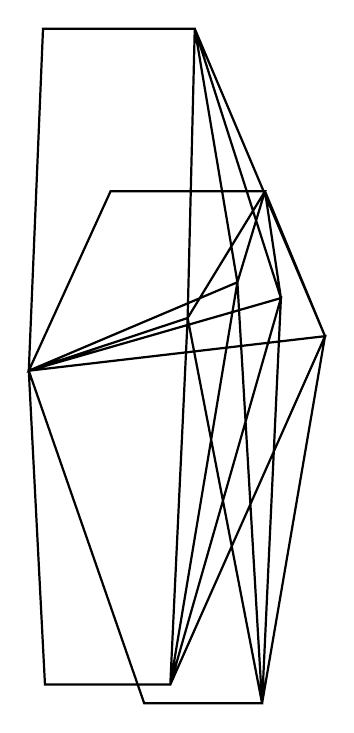
\begin{tikzpicture}
            \draw[thick](0,0)(0,0)  -- (0.18079912028074951, 4.342461501176299) -- (2.1079880947940572, 4.342461501176299) -- (2.0174410579488695,0.6694481151048982) -- (0,0) -- (0,0)  -- (0.20564447575375056, -3.9862913214253948) -- (1.7972376466289879, -3.9862913214253948) -- (2.0174410579488695,0.6694481151048982) -- (0,0) -- 
(0,0)  -- (0.18079912028074951, 4.342461501176299) -- (2.1079880947940572, 4.342461501176299) -- (2.0174410579488695,0.6694481151048982) -- (0,0) -- (0,0)  -- (1.4661311082797228, -4.22456748471439) -- (2.9628613597796845, -4.22456748471439) -- (2.0174410579488695,0.6694481151048982) -- (0,0) -- 
(0,0)  -- (1.0387477566426715, 2.2789653436643156) -- (2.999746862486046, 2.2789653436643156) -- (2.0174410579488695,0.6694481151048982) -- (0,0) -- (0,0)  -- (0.20564447575375056, -3.9862913214253948) -- (1.7972376466289879, -3.9862913214253948) -- (2.0174410579488695,0.6694481151048982) -- (0,0) -- 
(0,0)  -- (1.0387477566426715, 2.2789653436643156) -- (2.999746862486046, 2.2789653436643156) -- (2.0174410579488695,0.6694481151048982) -- (0,0) -- (0,0)  -- (1.4661311082797228, -4.22456748471439) -- (2.9628613597796845, -4.22456748471439) -- (2.0174410579488695,0.6694481151048982) -- (0,0) -- 
(0,0)  -- (0.18079912028074951, 4.342461501176299) -- (2.1079880947940572, 4.342461501176299) -- (3.2021711110418996,0.9221220355124299) -- (0,0) -- (0,0)  -- (0.20564447575375056, -3.9862913214253948) -- (1.7972376466289879, -3.9862913214253948) -- (3.2021711110418996,0.9221220355124299) -- (0,0) -- 
(0,0)  -- (0.18079912028074951, 4.342461501176299) -- (2.1079880947940572, 4.342461501176299) -- (3.2021711110418996,0.9221220355124299) -- (0,0) -- (0,0)  -- (1.4661311082797228, -4.22456748471439) -- (2.9628613597796845, -4.22456748471439) -- (3.2021711110418996,0.9221220355124299) -- (0,0) -- 
(0,0)  -- (1.0387477566426715, 2.2789653436643156) -- (2.999746862486046, 2.2789653436643156) -- (3.2021711110418996,0.9221220355124299) -- (0,0) -- (0,0)  -- (0.20564447575375056, -3.9862913214253948) -- (1.7972376466289879, -3.9862913214253948) -- (3.2021711110418996,0.9221220355124299) -- (0,0) -- 
(0,0)  -- (1.0387477566426715, 2.2789653436643156) -- (2.999746862486046, 2.2789653436643156) -- (3.2021711110418996,0.9221220355124299) -- (0,0) -- (0,0)  -- (1.4661311082797228, -4.22456748471439) -- (2.9628613597796845, -4.22456748471439) -- (3.2021711110418996,0.9221220355124299) -- (0,0) -- 
(0,0)  -- (0.18079912028074951, 4.342461501176299) -- (2.1079880947940572, 4.342461501176299) -- (3.7621853686773328,0.43856555968563127) -- (0,0) -- (0,0)  -- (0.20564447575375056, -3.9862913214253948) -- (1.7972376466289879, -3.9862913214253948) -- (3.7621853686773328,0.43856555968563127) -- (0,0) -- 
(0,0)  -- (0.18079912028074951, 4.342461501176299) -- (2.1079880947940572, 4.342461501176299) -- (3.7621853686773328,0.43856555968563127) -- (0,0) -- (0,0)  -- (1.4661311082797228, -4.22456748471439) -- (2.9628613597796845, -4.22456748471439) -- (3.7621853686773328,0.43856555968563127) -- (0,0) -- 
(0,0)  -- (1.0387477566426715, 2.2789653436643156) -- (2.999746862486046, 2.2789653436643156) -- (3.7621853686773328,0.43856555968563127) -- (0,0) -- (0,0)  -- (0.20564447575375056, -3.9862913214253948) -- (1.7972376466289879, -3.9862913214253948) -- (3.7621853686773328,0.43856555968563127) -- (0,0) -- 
(0,0)  -- (1.0387477566426715, 2.2789653436643156) -- (2.999746862486046, 2.2789653436643156) -- (3.7621853686773328,0.43856555968563127) -- (0,0) -- (0,0)  -- (1.4661311082797228, -4.22456748471439) -- (2.9628613597796845, -4.22456748471439) -- (3.7621853686773328,0.43856555968563127) -- (0,0) -- 
(0,0)  -- (0.18079912028074951, 4.342461501176299) -- (2.1079880947940572, 4.342461501176299) -- (2.649410212545587,1.123148269293016) -- (0,0) -- (0,0)  -- (0.20564447575375056, -3.9862913214253948) -- (1.7972376466289879, -3.9862913214253948) -- (2.649410212545587,1.123148269293016) -- (0,0) -- 
(0,0)  -- (0.18079912028074951, 4.342461501176299) -- (2.1079880947940572, 4.342461501176299) -- (2.649410212545587,1.123148269293016) -- (0,0) -- (0,0)  -- (1.4661311082797228, -4.22456748471439) -- (2.9628613597796845, -4.22456748471439) -- (2.649410212545587,1.123148269293016) -- (0,0) -- 
(0,0)  -- (1.0387477566426715, 2.2789653436643156) -- (2.999746862486046, 2.2789653436643156) -- (2.649410212545587,1.123148269293016) -- (0,0) -- (0,0)  -- (0.20564447575375056, -3.9862913214253948) -- (1.7972376466289879, -3.9862913214253948) -- (2.649410212545587,1.123148269293016) -- (0,0) -- 
(0,0)  -- (1.0387477566426715, 2.2789653436643156) -- (2.999746862486046, 2.2789653436643156) -- (2.649410212545587,1.123148269293016) -- (0,0) -- (0,0)  -- (1.4661311082797228, -4.22456748471439) -- (2.9628613597796845, -4.22456748471439) -- (2.649410212545587,1.123148269293016) -- (0,0) -- 
(0,0);
            \end{tikzpicture}
            \end{center}
            \caption{Square of the complex, with edges $(g,ag), (agb, gb) \in E_A,
            (g,gb), (agb, ag) \in E_B.$ \label{fig:square}
            }
            \end{figure}
 
\end{multicols*}
  % \printbibliography 
\end{document}

 